\documentclass[handout]{beamer}

\usetheme{Warsaw}
\usefonttheme[onlylarge]{structurebold}
\useinnertheme{rectangles}
\setbeamerfont*{frametitle}{size=\normalsize,series=\bfseries}
\setbeamertemplate{navigation symbols}{}

\usepackage[polish]{babel}
\usepackage[utf8]{inputenc}
\usepackage{times}
\usepackage[T1]{fontenc}
\usepackage{listings}
\usepackage{graphicx}
\usepackage{enumerate}
\usepackage{tikz}
\usepackage[normalem]{ulem}
\usepackage{bussproofs}

\definecolor{ugreen}{rgb}{0, 0.5, 0}
\definecolor{lgreen}{rgb}{0.85, 1, 0.85}
\definecolor{annot}{rgb}{0.7, 0, 0}
\definecolor{lstback}{RGB}{235 240 250}

\setbeamercolor{gr}{fg=white, bg=ugreen}
\setbeamercolor{lgr}{fg=black, bg=lgreen}

\setcounter{tocdepth}{1}
\AtBeginSection[]
{
  \begin{frame}<beamer>{Plan}
    \tableofcontents[currentsection, hideothersubsections]
  \end{frame}
}

\title{Weryfikacja funkcyjności metod Javy}

\author{Sławomir Rudnicki} 

\institute{Niezawodność systemów współbieżnych i obiektowych}

\date{16 marca 2011}

\lstset{language=Java, showstringspaces=false, backgroundcolor=\color{lstback}, 
        emph={@Pure, @Function}, 
        morekeywords={assert}, 
        emphstyle={\color{annot}}, 
        columns=fullflexible}

\begin{document}

\begin{frame}
  \titlepage
\end{frame}
\begin{frame}
  \tableofcontents[pausesections]
\end{frame}

\setcounter{tocdepth}{2}

\section{Wprowadzenie}

\begin{frame}{Wprowadzenie}
  Dla danej metody w Javie sprawdzamy pewne własności wprowadzone
  przez adnotacje \pause \lstinputlisting{code/intro-annot.java}
\end{frame}

\section{Własności funkcyjności metod}

\subsection{Czysta funkcyjność}

\begin{frame}{Czysta funkcyjność}
  Metoda czysto funkcyjna (ang. \textsl{pure}):
  \begin{itemize}
  \item nie posiada efektów ubocznych, czyli:
  \item nie modyfikuje stanu obiektów
  \end{itemize}
\end{frame}

\begin{frame}{Czysta funkcyjność}
  Czy ta metoda jest czysto funkcyjna?
  \lstinputlisting{code/sum.java}
\end{frame}

\begin{frame}{Czysta funkcyjność}
  Metoda czysto funkcyjna (ang. \textsl{pure}):
  \begin{itemize}
  \item nie posiada efektów ubocznych
  \item nie modyfikuje stanu obiektów \alert{istniejących na stercie w momencie jej wywołania}
  \end{itemize}
\end{frame}

\begin{frame}{Po co nam czysta funkcyjność?}
  \begin{itemize}
    \item Metody czysto funkcyjne mogą być używane w specyfikacji i asercjach:
  \end{itemize}
  \lstinputlisting{code/assertion.java}
\end{frame}

\begin{frame}{Po co nam czysta funkcyjność?}
  Metody czysto funkcyjne:
  \begin{itemize}
  \item<1-> mogą być wywoływane współbieżnie
    \begin{itemize}
    \item w szczególności niemożliwe są wyścigi o dane (\textsl{data race})
    \item w weryfikacji opartej o przeszukiwanie przestrzeni stanów 
      można pominąć analizę przeplotów pomiędzy dwiema metodami
      czysto funkcyjnymi
    \end{itemize}
  \item<2-> nie naruszają niezmienników systemu
  \item<3-> mogą być wywoływane bez szkody dla integralności 
    pozostałej części systemu, nawet jeśli są niezaufane. 
  \end{itemize}
\end{frame}

\subsection{Funkcyjność deterministyczna}

\begin{frame}{Funkcyjność deterministyczna}
  Metoda deterministycznie funkcyjna:
  \begin{itemize}
  \item jest czysto funkcyjna
  \item wywołana z \alert<2>{tymi samymi} argumentami, zawsze daje ten sam wynik
  \end{itemize}
\end{frame}

\begin{frame}{Po co nam funkcyjność deterministyczna?}
  \begin{itemize}
  \item Metoda funkcyjna może być bezpiecznie wywoływana w środowisku
    wielowątkowym.
  \item W asercjach determinizm zapewnia powtarzalność błędów i 
    poprawnych wykonań.
  \item Wykonanie metody funkcyjnej jest powtarzalne
    \begin{itemize}
    \item Przydatne w systemach z historią działania.
    \item Zapewnia ważne własności bezpieczeństwa.
    \end{itemize}
  \end{itemize}
\end{frame}

\begin{frame}{Po co nam funkcyjność deterministyczna?}
  \begin{center}
    Elektroniczny system głosowania
  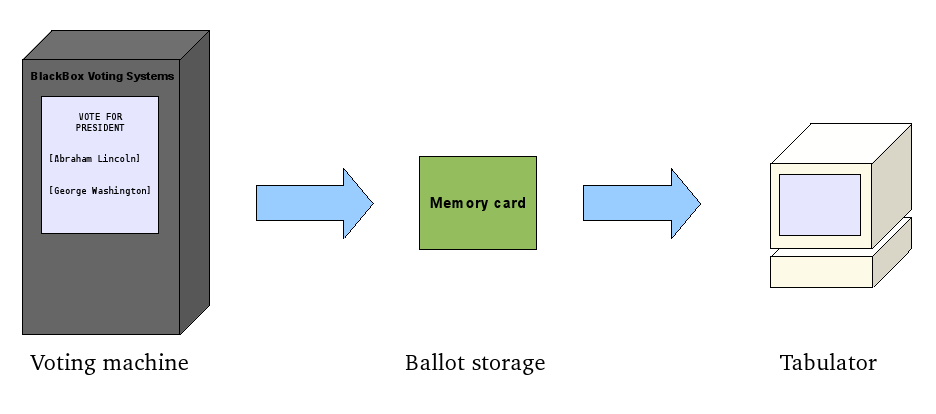
\includegraphics[width=\columnwidth]{img/voting-1.png}
  \end{center}
\end{frame}

\begin{frame}{Po co nam funkcyjność deterministyczna?}
  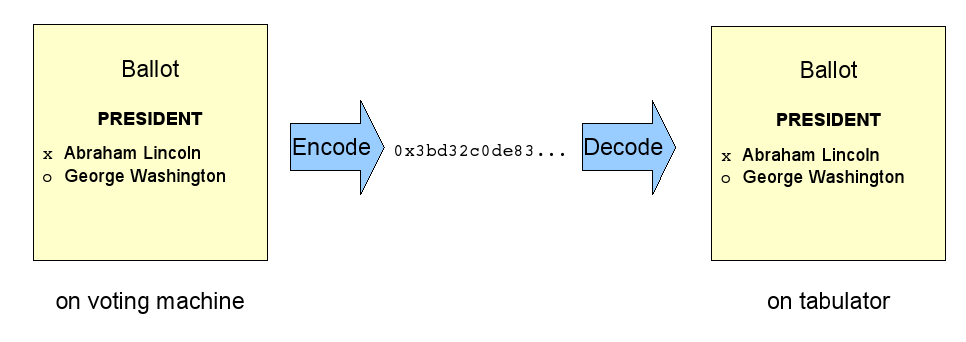
\includegraphics[width=\columnwidth]{img/voting-2.png}
  \begin{center}
  \pause
  Jak zapewnić, że głos zostanie poprawnie przeliczony? \\
  \pause
  \texttt{\textbf{assert}(x == decode(y));} \\
  \pause
  \alert{\texttt{decode} musi być funkcyjna}
  \end{center}
\end{frame}

\section{Weryfikacja czystej funkcyjności}

\subsection{Wprowadzenie}

\begin{frame}{Weryfikacja czystej funkcyjności}
  Metoda -- \textbf{Analiza statyczna}
  \begin{itemize}
    \item dla każdego punktu sterowania
    budujemy strukturę wskaźników, która reprezentuje część sterty
    widoczną dla metody do tego punktu.
  \end{itemize}
  \pause
  Podstawowe problemy:
  \begin{itemize}
  \item<2-> Śledzenie nowo utworzonych obiektów
    \begin{itemize}
    \item Tylko one mogą być modyfikowane
    \end{itemize}
  \item<3-> Wywołania innych metod
    \begin{itemize}
    \item Jak zmieniają strukturę?
    \end{itemize}
  \end{itemize}
  \pause
\end{frame}

\subsection{Analiza przepływu danych}

\begin{frame}{Analiza przepływu danych -- ogólnie}
\begin{center}
  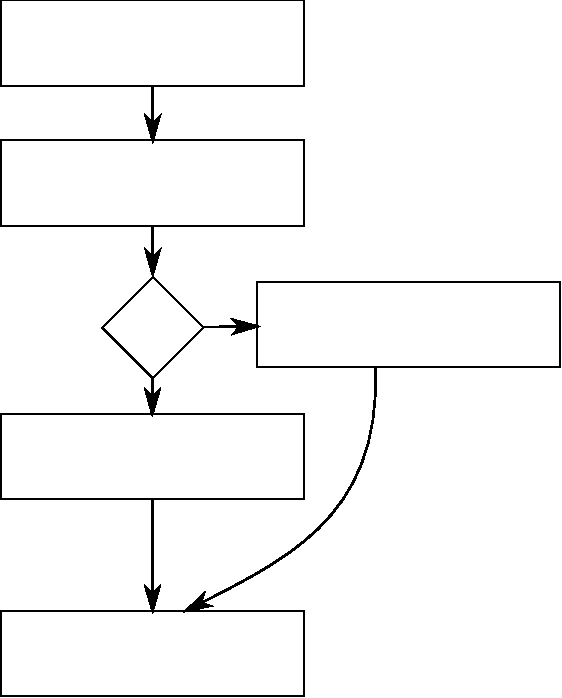
\includegraphics[scale=0.55]{img/dataflow.pdf}  
\end{center}
\end{frame}

\begin{frame}{Analiza przepływu danych -- ogólnie}
\begin{center}
  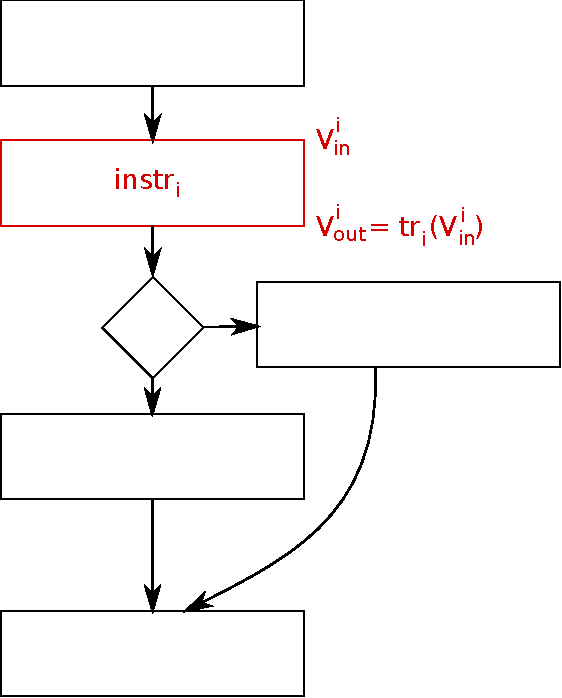
\includegraphics[scale=0.55]{img/dataflow-1.pdf}  
\end{center}
\end{frame}

\begin{frame}{Analiza przepływu danych -- ogólnie}
\begin{center}
  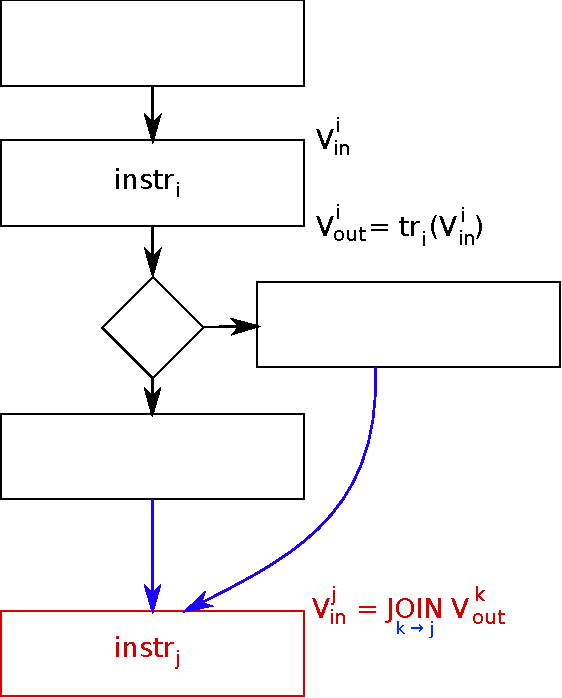
\includegraphics[scale=0.55]{img/dataflow-2.pdf}  
\end{center}
\end{frame}

\subsection{Graf wskaźników}

\begin{frame}
  Dla każdego punktu sterowania utrzymujemy:
  \begin{enumerate}
  \item<1-> graf wskaźników (ang. \emph{points-to graph})
  \item<1-> zbiór pól, które \emph{uciekają} z metody
      $$G = \left<I, O, L, E\right>$$
  \item<2-> zbiór modyfikowanych pól
    $$W = \mathcal{P}\left(Node \times Field\right)$$
  \end{enumerate}
\end{frame}

\begin{frame}{Graf wskaźników: konwencje}
  \tikzstyle{init} = [pin edge={to-,thin,black}]
  \begin{itemize}
  \item Węzeł wewnętrzny -- utworzony w metodzie 
    \begin{center} 
      \tikz \node[draw, circle]{P};
    \end{center}
  \item Węzeł zewnętrzny -- odczytany w metodzie 
    \begin{center}
      \tikz \node[draw, circle, dashed]{P};
    \end{center}
  \item Krawędź wewnętrzna -- utworzona w metodzie:
    \begin{center}
      \begin{tikzpicture}[node distance=1.5in, auto]
        \node [draw, circle] (a) {$n_1$};
        \node [draw, circle] (b) [right of=a] {$n_2$};
        \path[->] (a) edge node {$f$} (b);
      \end{tikzpicture}
    \end{center}
  \item Krawędź zewnętrzna -- odczytana w metodzie: 
    \begin{center}
      \begin{tikzpicture}[node distance=1.5in, auto]
        \node [draw, circle, dashed] (a) {$n_1$};
        \node [draw, circle, dashed] (b) [right of=a] {$n_2$};
        \path[->] [dashed] (a) edge node {$f$} (b);
      \end{tikzpicture}
    \end{center}
  \end{itemize}
\end{frame}

\begin{frame}{Przykładowy graf wskaźników}
  \begin{columns}[l]
    \column{1.5in}
    \lstinputlisting{code/ptg-example.java}
    \column{1.5in}
    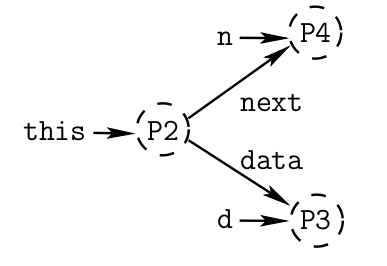
\includegraphics[scale=0.4]{img/ptg-example.png}
    $$W = \lbrace\left<P2, \text{data}\right>, \left<P2, \text{next}\right>\rbrace$$
  \end{columns}
\end{frame}

\begin{frame}{Funkcja transferu}
  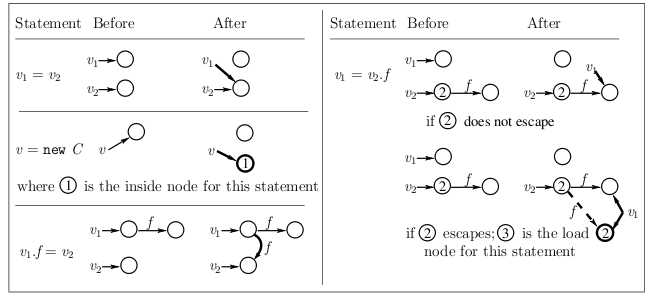
\includegraphics[width=\columnwidth]{img/transfer.png}
\end{frame}

\begin{frame}{Wołanie metod}
  $$v_R = v_0.s(v_1, \dots, v_j)$$
  \begin{itemize}
    \item<1-> metody nieanalizowalne
      \begin{itemize}
        \item $v_R$ jest nieznane, 
        \item $v_i$ uciekają
      \end{itemize}
    \item<2-> metody analizowalne
      \begin{enumerate}
        \item mapowanie węzłów z grafu metody wołanej
        \item połączenie grafów
        \item uproszczenie grafu wynikowego
      \end{enumerate}
  \end{itemize}
\end{frame}

\begin{frame}{Wołanie metod: mapowanie węzłów}
  $$\mu' \subseteq Node \times Node$$
  \begin{itemize}
  \item dla węzła $n$ z grafu wskaźników dla metody wołanej, $\mu'(n)$
    zawiera odpowiadające mu węzły z grafu po wywołaniu metody.
  \end{itemize}
\end{frame}

\begin{frame}{Wołanie metod: konstrukcja mapowania}
  \begin{enumerate}
    \item<1-> $\forall i\in\lbrace1\dots j\rbrace\quad L(v_i) \subseteq \mu\left(n_{callee,i}^{P}\right)$
    \item<2-> $\quad$
      \begin{prooftree}
        \AxiomC{$\left<n_1, f, n_2\right> \in O_{callee} \quad \left<n_3, f, n_4\right>\in I \quad n_3 \in \mu(n_1)$}
        \UnaryInfC{$n_4 \in \mu(n_2)$}
      \end{prooftree}
      \visible<3->{
      \begin{center}
        \begin{tikzpicture}[node distance=1.5in, auto, >=stealth]
          \node [draw=red, circle, dashed] (a) {$n_1$};
          \node [draw=red, circle, dashed] (b) [right of=a] {$n_2$};
          \path[->] [dashed, draw=red] (a) edge node {$f$} (b);
          \node [draw=blue, circle] (c) [below of=a, node distance=1in] {$n_3$};
          \node [draw=blue, circle] (d) [below of=b, node distance=1in] {$n_4$};
          \path[->] [draw=blue] (c) edge node {$f$} (d);
          \path[->] [dotted] (a) edge (c);
          \only<4->{\path[->] [very thick] (b) edge (d);}
        \end{tikzpicture}
      \end{center}
      }
  \end{enumerate}
\end{frame}

\begin{frame}{Wołanie metod: konstrukcja mapowania}
  \begin{enumerate}
    \setcounter{enumi}{2}
    \item 
      \begin{prooftree}
        \AxiomC{$\left<n_1, f, n_2\right> \in O_{callee}\quad \left<n_3, f, n_4\right>\in I_{callee}$}
        \noLine
        \UnaryInfC{$\left(\mu(n_1) \cup \lbrace n_1\rbrace\right) 
          \cap \left(\mu(n_3) \cup \lbrace n_3\rbrace\right) \neq \emptyset$}
        \UnaryInfC{$\mu(n_4) \cup\left(\lbrace n_4\rbrace \setminus PNode\right) \subseteq\mu(n_2)$}
      \end{prooftree}
      \hspace{1in}
        \begin{tikzpicture}[node distance=1.5in, auto, >=stealth]
          \node [draw=red, circle, dashed] (a) {$n_1$};
          \node [draw=red, circle, dashed] (b) [right of=a] {$n_2$};
          \path[->] [dashed, draw=red] (a) edge node {$f$} (b);
          \node [draw=red, circle, dashed] (c) [below of=a, node distance=0.7in]{$n_3$};
          \node [draw=red, circle, dashed] (d) [below of=b, node distance=0.7in] {$n_4$};
          \path[->] [draw=red] (c) edge node {$f$} (d);
          \node [draw=blue, circle] (e) [below of=c, node distance=0.7in] {$n_5$};
          \node [draw=blue, circle] (f) [below of=d, node distance=0.7in] {$n_6$};
          \path[->] [dotted, bend right] (c) edge (e);
          \path[->] [dotted, bend right] (a) edge (e);
          \path[->] [dotted] (d) edge (f);
          \only<2->{
            \path[->] [very thick, bend left] (b) edge (d);
          }
          \only<3->{
            \path[->] [very thick, bend left] (b) edge (f);
          }
        \end{tikzpicture}
      %\end{center}
  \end{enumerate}
\end{frame}

\begin{frame}{Wołanie metod: konstrukcja mapowania}
  \begin{itemize}
  \item iterujemy reguły 1-3 do uzyskania punktu stałego, 
  \item uzupełniamy $\mu$ do $\mu'$:
    $$\mu'(n) = \mu(n) \cup (\lbrace n\rbrace \setminus PNode)$$
  \end{itemize}
\end{frame}

\begin{frame}{Wołanie metod: inne szczegóły}
  \begin{itemize}
  \item<1-> Połączenie grafów:
    \begin{itemize}
    \item dodajemy krawędzie jak w wołanej metodzie
    \item uwzględniamy węzły \emph{uciekające} z metody wołanej
    \item do $W$ dodajemy te węzły, na które mapują się pola
      modyfikowane w wołanej metodzie
    \end{itemize}
  \item<2-> Uproszczenie grafu wynikowego:
    \begin{itemize}
    \item usuwamy \emph{schwytane} wierzchołki zewnętrzne
    \end{itemize}
  \end{itemize}
\end{frame}

\subsection{Przykład}

\begin{frame}{Przykład}
  \small{
    \lstinputlisting{code/example-1.java}
  }
\end{frame}

\begin{frame}{Przykład}
  \small{
    \lstinputlisting{code/example-2.java}
  }
\end{frame}

\begin{frame}{Przykład}
  Weryfikujemy czystą funkcyjność następującej funkcji: 
  \lstinputlisting{code/example-3.java}
\end{frame}

\begin{frame}{Wnioski z grafu wskaźników}
  \begin{itemize}
    \item \textbf{Czysta funkcyjność.}
      $A$ -- zbiór węzłów osiągalnych z parametrów przez krawędzie zewnętrzne, 
      $B$ -- zbiór węzłów osiągalnych z $E$. 
      Metoda jest czysto funkcyjna wtw:
      $$A \cap B = \emptyset$$
      oraz 
      $$\forall n \in A \neg\exists f \quad \left<n,f\right>\in W$$
  \end{itemize}
\end{frame}

\begin{frame}{Wnioski z grafu wskaźników}
  \begin{itemize}
    \item \textbf{Stałe parametry.}  $S_1$ -- osiągalne z parametru po
      krawędziach zewnętrznych. Parametr jest stały wtw.:
      $$\forall n \in S_1 \neg\exists f \quad \left<n,f\right>\in W$$
    \item \textbf{Bezpieczne parametry.} $S_2$ -- osiągalne z
      parametru i węzła zwracanego. Parametr jest bezpieczny wtw. jest
      stały i nie istnieje krawędź wewnętrzna ze zbioru $S_2$ do
      zbioru $S_1$
  \end{itemize}
\end{frame}

\begin{frame}{Wnioski z grafu wskaźników}
  \begin{itemize}
    \item \textbf{Modyfikowane pola} -- z grafu wskaźników tworzymy
      automat nad alfabetem złożonym z identyfikatorów, który będzie
      akceptował wszystkie i tylko słowa postaci $v.f_1.f_2.\cdots.f_n$
      takie, że wskazane pole jest modyfikowane w metodzie. 
  \end{itemize}
\end{frame}

\begin{frame}{Metoda grafu wskaźników -- podsumowanie}
  \begin{beamerboxesrounded}[upper=gr, lower=lgr, shadow=true]{\bf Zalety}
    \begin{itemize}
    \item Dokładne odwzorowanie fragmentu sterty widocznego w metodzie
    \item Możliwość wnioskowania o innych własnościach metody
    \item Możliwość wnioskowania własności, a nie tylko ich dowodzenia. 
    \end{itemize}
  \end{beamerboxesrounded}
  \pause
  \begin{alertblock}{Problemy}
    \begin{itemize}
    \item Analiza nie jest modularna -- do weryfikacji metody
      potrzebny jest kod źródłowy metod, które są z niej wywoływane.
    \end{itemize}
  \end{alertblock}
\end{frame}

\subsection{JPure}

\begin{frame}{JPure}
  Weryfikacja czystej funkcyjności sprawdzalna modularnie:
  \begin{itemize}
    \item Do weryfikacji danego pliku wystarczy jego kod źródłowy.
    \item Informacja o funkcyjności metod jest przekazywana 
      pomiędzy plikami źródłowymi przy użyciu adnotacji Javy:
      \pause
      \vspace{0.3in}
      \begin{center}
        \color{annot}{@Pure\hspace{0.8in}@Fresh\hspace{0.8in}@Local}
      \end{center}
  \end{itemize}
\end{frame}

\begin{frame}{Naiwne podejście}
  Sprawdzamy, czy metoda:
  \begin{itemize}
  \item nie modyfikuje bezpośrednio pól obiektów,
  \item nie woła metod, które nie są czysto funkcyjne, 
  \item nie implementuje lub redefiniuje metody zadeklarowanej jako
    czysto funkcyjna, sama nie będąc czysto funkcyjną.
  \end{itemize}
  \pause
  \begin{center}
    \alert{Dlaczego jest źle?}
  \end{center}
\end{frame}

\begin{frame}{Dlaczego jest źle?}
  \lstinputlisting{code/sum.java}
\end{frame}

\begin{frame}{Dlaczego jest źle?}
  Aby \textbf{getSum} była czysto funkcyjna, musielibyśmy wiedzieć, że:
  \begin{itemize}
    \item \textbf{l.iterator()} jest czysto funkcyjna i zwraca nowy
      obiekt, 
      \visible<2->{
        \begin{center}
          \textcolor{annot}{@Fresh} Iterator iterator();
        \end{center}
      }
    \item \textbf{it.hasNext()} oraz \textbf{it.next()} modyfikują 
      tylko obiekt \textbf{it}.
      \visible<3->{
        \begin{center}
          \textcolor{annot}{@Local} Integer next();
        \end{center}
      }
  \end{itemize}
\end{frame}

\begin{frame}{Adnotacje}
  \begin{itemize}
    \item \textbf{{\color{annot} @Local} na polu:} pole jest
      składnikiem stanu wewnętrznego obiektu.
    \item \textbf{{\color{annot} @Local} na parametrze} (w
      szczególności na odbiorcy): tylko stan wewnętrzny parametrów
      oznaczonych {\color{annot} @Local} może być modyfikowany.
    \item \textbf{{\color{annot} @Pure}:} metoda jest czysto funkcyjna.
    \item \textbf{{\color{annot} @Fresh}:} metoda jest czysto funkcyjna
      i zwraca nowy obiekt.
  \end{itemize}
\end{frame}

\begin{frame}{Weryfikacja adnotacji}
  \begin{itemize}
    \item {\color{annot} @Pure}:
      \begin{itemize}
        \item metoda nie modyfikuje nielokalnych parametrów, 
        \item metoda woła inne metody poprawnie ze względu na
          lokalność jej parametrów.
      \end{itemize}
    \item {\color{annot} @Fresh}: jw., poza tym metoda zwraca nowy
      obiekt.
  \end{itemize}
  \pause
  Weryfikacja wewnątrzproceduralna przy użyciu uproszczonego grafu
  wskaźników, przy założeniu, że adnotacje poza właśnie weryfikowaną
  metodą są poprawne.
\end{frame}

\begin{frame}{Wnioskowanie o czystej funkcyjności}
  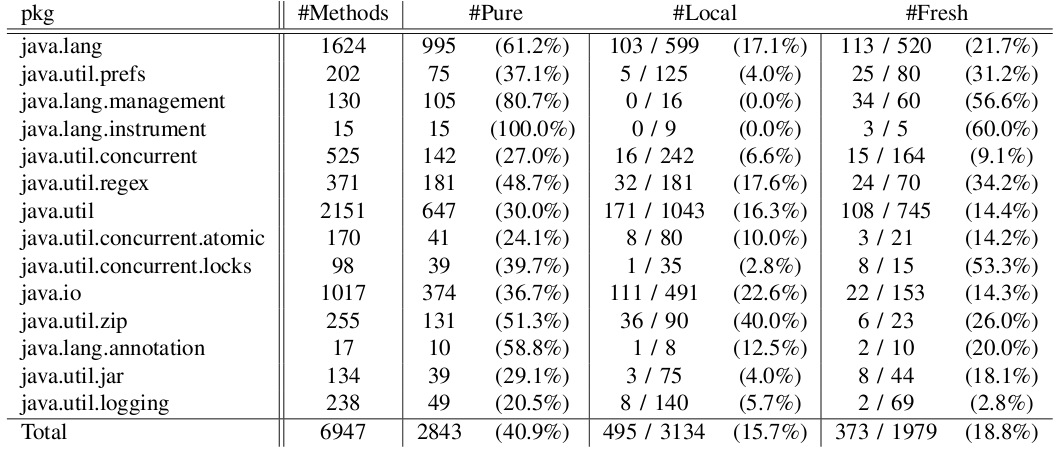
\includegraphics[width=\columnwidth]{img/experiment.png}
\end{frame}

\section{Funkcyjność deterministyczna}

\subsection{Joe-E}

\begin{frame}{Joe-E}
  Weryfikacja funkcyjności deterministycznej:
  \begin{itemize}
    \item wyróżniamy podzbiór Javy, który jest deterministycznym językiem
      obiektowo-uprawnieniowym (ang. \emph{object-capability language}), 
  \end{itemize}
\end{frame}

\begin{frame}{Język obiektowo-uprawnieniowy}
  \begin{itemize}
  \item<1-> Stan systemu jest w całości przechowywany w obiektach, 
  \item<2-> Obiekty są dostępne jedynie przez referencję, 
  \item<3-> Referencje mogą być przekazywane tylko:
    \begin{itemize}
      \item jako argumenty metod, 
      \item przez stan współdzielonych obiektów, 
    \end{itemize}
  \end{itemize}
  \pause
  Referencje modelują {\bf uprawnienia} obiektów do korzystania z
  innych obiektów.
\end{frame}

\begin{frame}{Język obiektowo-uprawnieniowy $\subseteq$ Java}
  Ten kod nie jest deterministyczny:
  \lstinputlisting{code/nondet.java}
  \pause
  ...a ten ma efekty uboczne:
  \lstinputlisting{code/sideef.java}
  \pause
  Pozwalamy wołać tylko niektóre funkcje z biblioteki standardowej.
\end{frame}

\begin{frame}{Joe-E}
  Weryfikacja funkcyjności deterministycznej:
  \begin{itemize}
    \item wyróżniamy podzbiór Javy, który jest językiem
      obiektowo-uprawnieniowym
    \item deterministyczną funkcyjność metody w takim języku 
      zapewnia:
      \begin{itemize}
      \item niemutowalność wszystkich jej parametrów i odbiorcy, 
      \item niemutowalność zmiennych statycznych.
      \end{itemize}
  \end{itemize}
\end{frame}

\begin{frame}{Joe-E -- implementacja}
  \begin{itemize}
  \item Niemutowalność:
    \begin{itemize}
    \item wprowadzana przez interfejs, 
    \item wymuszenie modyfikatora \texttt{final} na polach, 
    \item pola są typu prymitywnego lub są referencją do 
      obiektu typu niemutowalnego, 
    \item konstruktory nie mogą wołać metod instancyjnych. 
  \end{itemize}
  \item Funkcyjność:
    \begin{itemize}
      \item niemutowalność wszystkich parametrów
    \end{itemize}
  \end{itemize}
\end{frame}

\begin{frame}{Joe-E w praktyce}
  Weryfikator Joe-E został użyty do sprawdzenia deterministycznej
  funkcyjności:
  \begin{itemize}
  \item<1-> biblioteki AES
    \begin{itemize}
      \item szyfrowanie i deszyfrowanie
    \end{itemize}
  \item<2-> implementacji maszyn do głosowania 
    \begin{itemize}
      \item serializacja i deserializacja
    \end{itemize}
  \item<3-> parsera HTML
  \end{itemize}
\end{frame}

\begin{frame}{Joe-E -- podsumowanie}
  \begin{alertblock}{Problemy z Joe-E}
    \begin{itemize} 
    \item<1-> Niemutowalność obiektu wymaga niemutowalności wszystkich
      obiektów z niego osiągalnych, 
    \item<1-> Brak wyróżnienia stanu wewnętrznego i zewnętrznego obiektu, 
    \item<2-> Niemutowalność definiowana dla klas: brak pojęcia obiektu
      tylko do odczytu, 
    \item<3-> Kryterium czystości deterministycznej jest bardzo silne. 
    \end{itemize}
  \end{alertblock}
  \pause
  \begin{beamerboxesrounded}[upper=gr, lower=lgr, shadow=true]{\bf Wniosek:}
    Na pewno da się zrobić to lepiej!
  \end{beamerboxesrounded}
\end{frame}

\begin{frame}{Bibliografia}
  \begin{itemize}
  \item A. S\u{a}lcianu, M. Rinard, \\
    \emph{Purity and side-effect analysis for Java programs}, \\
         Proc. VMCAI, 2005, ss. 199--215.
  \item D. J. Pearce, \\
    \emph{JPure: A modular purity system for Java}, \\
    Proceedings of the Conference on Compiler Construction, 2011
  \item M. Finifter, A. Mettler, N. Sastry, D. Wagner, \\
    \emph{Verifiable functional purity in Java} \\
    Proc. CCS, ACM 2008, ss. 161--174.
  \end{itemize}
\end{frame}

\begin{frame}{Praca magisterska}
  Rozwój projektu i pracy można obserwować w publicznym repozytorium:
  \begin{center}
    \vspace{3mm}
    \structure{www.github.com/saf/Funcheck}\\
    \vspace{3mm}
    \texttt{git clone git://github.com/saf/Funcheck.git}
  \end{center}
\end{frame}

\end{document}

